
\chapter{Limpieza de datos: extracción de usuarios relevantes}
\label{chap:extraccion_de_usuarios}

Como hemos visto en el análisis exploratorio inicial de los datos, para conseguir
nuestro objetivo final la fase de limpieza de la información va a ser muy relevante.
Se trata de extraer, a partir de los tuits almacenados, una lista de usuarios 
que pudieran constituirse en candidatos adecuados a una oferta de trabajo (como, por ejemplo, las de la figura \ref{fig:ofertas_descripcion}). Para ello, de todos aquellos usuarios de los
que tenemos constancia en los tuits recogidos hemos de seleccionar aquellos que sean personas (eliminando bots, empresas, etc.) y que hayan publicado contenido relacionado con la materia de referencia, en este caso la ciencia de datos.



\subsection{Detección del idioma} 

El primer paso para poder analizar el contenido de un tuit y determinar si dicho tuit (y por tanto el usuario que lo ha publicado) está relacionado con la ciencia de datos o el big data,
es determinar el lenguaje en el que está escrito. Como ya hemos mencionado,
aunque la búsqueda en Twitter se realizó solicitando el campo \lq\lq languages = ["es"]\rq\rq,
obtenemos algunos tuits en otros idiomas, como estos dos 
que mostramos a continuación:

\myfigure{
\begin{tabular}{cc}

\includegraphics[width=0.4\textwidth]{tuit_ingles1}
&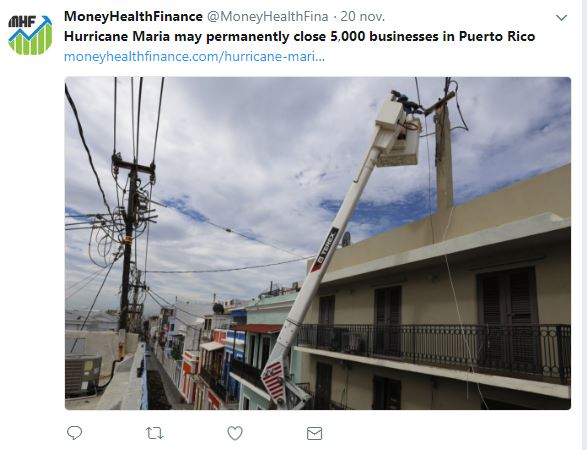
\includegraphics[width=0.4\textwidth]{tuit_ingles2}
\end{tabular}
\figcaption{Tuits no solo en español.}
\label{fig:tuits_ingles} }

Los primeros trabajos sobre el problema de la detección automática del lenguaje de un texto
se remontan a la década de 1970 \cite{zissman-berkling}. En la mayoría de las propuestas, existe una fase de entrenamiento, sobre textos previamente clasificados, en la que se produce un modelo del lenguaje (tal vez uno por lenguaje), y una fase de reconocimiento, en la que el lenguaje de mayor verosimilitud para el texto se extrae a partir de la aplicación de los distintos modelos. La clave de todos estos métodos es la modelización del lenguaje, cosa que puede conseguirse atendiendo a diversas características diferenciadoras: fonemas, morfología, sintaxis y/o prosodia.



\subsection{Tipo de usuario}
persona, bot, empresa análisis bio

\subsection{Naturaleza del tuit}
texto del tuit:  IT, cientifico, analista o nodatascience (diccionarios de palabras)
					/Binario, data science o no data science
